\usepackage[toc,page]{appendix}
\chapter{Design and Framework}
\section{System Design}
\begin{sidewaysfigure}
    \centerline{
    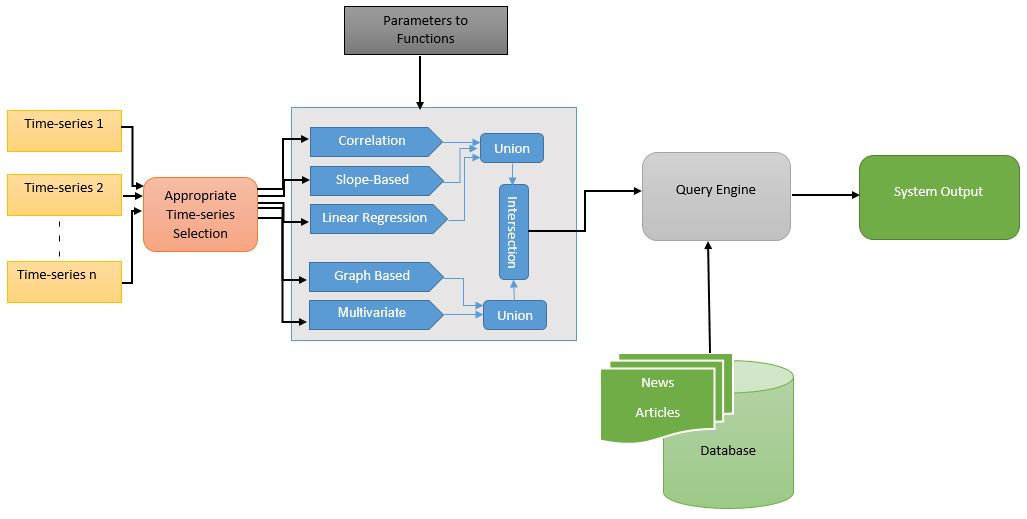
\includegraphics[width=0.9\textwidth]{System_updated.JPG}
    }
    \caption{System Framework}
    \label{fig:SystemDesign}
\end{sidewaysfigure}

Figure \ref{fig:SystemDesign} explains the overall design of the system and its modules.\\
\\
We have multiple time-series as input. These time-series are to be read from file manually using python script and generate 2D list of the time-series. These 2D lists has first column as date and then we have one or more columns corresponding to one or more values for that date. In the next stage depending upon what time-series we need to compare, we select appropriate time-series and pass this as input to various functions. Note that it is required to have all time-series of equal length and time period for which time-series are considered should be same for all time-series.\\
\\
We have implemented 5 functions till now as shown in figure \ref{fig:SystemDesign} viz. Correlation, Slope Based, Linear Regression, Graph Based and Multivariate. Detail about each function is explained in the next section. These functions takes either 2 or multiple time-series as input and has various parameters. Depending upon how time-series should behave with respect to each other (directly propotional or inversaly propotional) parameteres are tuned. We take union of results of first three functions and rest of the two functions as shown in figure. After taking union, we take intersection of two results of union as shown in figure. This is final result produced by the system. This result states the anomalies in the time-series.\\
\\
To verify result produced by system, we match it with the news articles present for the test case considered (here onion test case). We match system results with news articles present and check how well system is performing. Note that it is not necessary that for each and every anomaly case, we have news article present. If not, then we manually check behavior of time-series on that date. If some news articles do not match with system result then we also study, why they did not match and what are limitations of system.\\

\section{Anomaly Detection Library}
Following methods are implemented in the library to detect anomalies in given timeseries:
\subsection{Window Based Correlation}
The method finds anomalies between two timeseries. If the two timeseries are supposed to be positively correlated, then it reports all the tenures where the timeseries deviates from showing positive correlation between them.
\\
Similarly if the two timeseries are supposed to be negatively correlated, then it reports all the tenures where the timeseries deviates from showing negative correlation between them. The significant deviations are reported based on either the default significance value of 0.01 or it can be customized based on the need. For more information 
\subsection{Slope Based Detection}
The  method calculates the rate of change of one timeseries with respect to the other. The tenures are reported where one timeseries varies to a large extent from the other.
\\
The threshold is decided based on the MAD outlier detection test or it could be set manually.
\subsection{Linear Regression}
The method builds a linear model between two timeseries. Values are predicted based on this linear model and error is calulated. All the tenures with error values breaching the threshold are reported as anomaly. 
\\
The threshold can be decided by MAD outlier detection technique or it can be configured manually.
\subsection{Graph Based Anomaly}
Graph based anomaly detection technique considers each day as a node of a graph. Similar nodes are connected to each other by some weight. Similarity of nodes are calculated by making use of the values of that node i.e. value(s) of timeseries on that date. Based on this similarity, edge weights are also assigned. Then random walk algorithm is applied on this graph structure and connectivity value of each node is calculated. Graph nodes having the least connectivity values are reported as anomaly.
\\
The method also takes into account the trend, seasonality etc of timeseries. Top few points (can be configured) are reported as anomaly by the system.
\subsection{Multivariate- Vector Autoregressive}
The method uses vector autoregressive framework for multivariate time-series analysis in order to forecast values. The framework treats all the variables as symmetrical and all the variables are modeled as if they influence each others equally.
\\
Error percentage is calculated between actual and forecasted values. These error values are used to filter anomalous conditions from non-anomalous conditions by setting a threshold value which can be automatically computed by MAD outlier detection test or it can be manually configured to the required value.
\section{Hypothesis Testing}
These methods can be used for testing various hypothesis by changing the parameters in the library functions. The details are as following:
\begin{itemize}

\item Hypothesis 1: If the two timeseries are expected to be not in tandem then the tenures where they don't, needs to be reported as anomaly. It can be tested using above mentioned methods by changing some parameters. The details as follows:
 \begin{itemize}
   \item Window based correlation: positive\_correlation needs to be set to false. default\_threshold is set to true if user wants threshold to be decided by MAD outlier detection test otherwise it is set to false and the threshold is passed.
    \item Slope Based Detection: what\_to\_consider is set to -1. default\_threshold is set to true if user wants threshold to be decided by MAD outlier detection test otherwise it is set to false and the threshold is passed.
    \item Linear Regression: param is set to 1 in order to consider all the positive error values. default\_threshold is set to true if user wants threshold to be decided by MAD outlier detection test otherwise it is set to false and the threshold is passed.
  \end{itemize}

\item Hypothesis 2: If the two timeseries are expected to be in tandem then the tenures where they don't, needs to be reported as anomaly. It can be tested using above mentioned methods by changing some parameters. The details as follows:
  \begin{itemize}
   \item Window based correlation: positive\_correlation needs to be set to true. default\_threshold is set to true if user wants threshold to be decided by MAD outlier detection test otherwise it is set to false and the threshold is passed.
    \item Slope Based Detection: what\_to\_consider is set to 1. default\_threshold is set to true if user wants threshold to be decided by MAD outlier detection test otherwise it is set to false and the threshold is passed.
    \item Linear Regression: param is set to 1 in order to consider all the positive error values. default\_threshold is set to true if user wants threshold to be decided by MAD outlier detection test otherwise it is set to false and the threshold is passed.
  \end{itemize}
  
\item Hypothesis 3: Trend and seasonality in the data are to be taken care for this case. Following two methods are used:
    \begin{itemize}
      \item Graph Based Anomaly- numOfPtsReqd is set to get the required number of anomalous points.
      \item Multivariate- Vector Autoregressive- All the points which does not fall in the range of threshold are reported.
    \end{itemize}
    
\item Hypothesis 4:
    \begin{itemize}
      \item Since the slope based detection, window based detection and linear regression methods works only on the two timeseries at a time. So, in order to compare all the centres in one go, average of the timeseries of centers is computed and used for anomlay detection. 
      \item For Graph based and multivaraite- autoregressive anomaly detection methods, all the timeseries of centers are used to find anomalies.
    \end{itemize}
    

\end{itemize}

\textbf{Note (Applicable to Onion Case):} Results returned by H1 and H2, consists of all the time periods where arrival-wholesale price and wholesale price-retail price pairs go out of line. There may be case where, for each time of that year it may be going out of line and might not be anomaly. So, to remove such false positives, we can take intersection of results of H1 and results of H3. Similar thing can be done with H2 also, by taking  intersection of results of H2 and results of H3.

